\documentclass[a4paper,12pt]{article}  % standard LaTeX, 12 point type
\usepackage{geometry}
\usepackage{amsfonts,latexsym}
\usepackage{amsthm}
\usepackage{amssymb}
\usepackage[utf8]{inputenc} % Кодировка
\usepackage[english,russian]{babel} % Многоязычность

\newtheorem{theorem}{Theorem}[section]
\newtheorem{proposition}[theorem]{Proposition}
\newtheorem{lemma}[theorem]{Lemma}
\newtheorem{corollary}[theorem]{Corollary}
\newtheorem{conjecture}[theorem]{Conjecture}

\theoremstyle{definition}
\newtheorem{definition}{Определение}[section]
\newtheorem{example}{Example}[section]

% unnumbered environments:

\theoremstyle{remark}
\newtheorem*{remark}{Remark}
\newtheorem*{notation}{Notation}
\newtheorem*{note}{Note}

\setlength{\parskip}{5pt plus 2pt minus 1pt}
%\setlength{\parindent}{0pt}

\usepackage{color}
\usepackage{listings}
\usepackage{caption}
\usepackage{graphicx}
\usepackage{ucs}

\graphicspath{{pics/}}

\geometry{left=2cm}
\geometry{right=1.5cm}
\geometry{top=2cm}
\geometry{bottom=2cm}


\lstnewenvironment{algorithm}[1][]
{   
    \lstset{ 
        frame=tB,
        numbers=left, 
        mathescape=true,
        numberstyle=\small,
        basicstyle=\small, 
        inputencoding=utf8, 
        extendedchars=\true,
        keywordstyle=\color{black}\bfseries,
        keywords={,function, procedure, return, datatype, function, in, if, else, for, foreach, while, denote, do, and, then, assert,} 
        numbers=left,
        xleftmargin=.04\textwidth,
        #1 % this is to add specific settings to an usage of this environment (for instnce, the caption and referable label)
    }
}
{}

\newcommand{\tab}[1][0.3cm]{\ensuremath{\hspace*{#1}}}





\title{Modification of modificated CYK}
\author{Anya Yaveyn}
\date{\today}

\begin{document}


В работе~\cite{okhotin13} предложен модифицированный вариант алгоритма Валианта~\cite{valiant75} для синтаксического анализа, основанный на перемножении матриц. 
Основным недостатком этого алгоритма является сложность разделения его на независимые потоки. Нами предложена модификация этого алгоритма, которая отчасти решает эту проблему. Описание этой модификации разделено на несколько этапов: в разделе~\ref{se:term} введена терминология, немного отличающаяся от той, что используется в статье~\cite{okhotin13}. Далее, в разделе~\ref{se:okhotin} переформулирован оригинальный алгоритм в рамках этой терминологии. Разработанная модификация алгоритма описана в секции~\ref{se:modification}. В секции~\ref{se:parallel} обсуждаются возможности параллельной реализации исходного и модифицированного алгоритмов.



\section{Терминология}
\label{se:term}

Пусть $G=(\Sigma, N, R, S)$ --- контекстно-свободная грамматика в нормальной форме Хомского и $w = a_1 \dots a_{n}$ --- строка, причем $n + 1 = 2^k$. С некоторыми изменениями алгоритм, предложенный в работе~\cite{okhotin13}, применим также для булевых и стохастических грамматик. Подробнее адаптация алгоритма для использования с другими типами грамматик рассмотрена в статье \cite{okhotin13} и здесь отдельно рассматриваться не будет. Ограничение на длину строки (для обоих рассмотренных алгоритмов) введены скорее из соображений простоты изложения, так как оба алгоритма довольно легко обобщаются на строки произвольной длины. 

\begin{definition}
Пусть $G = (\Sigma, N, R, S)$ --- контекстно-свободная грамматика, а $A \in N$ --- нетерминальный символ, принадлежащий этой грамматике. Тогда определим $L_G(A) \subset \Sigma^\ast$, как язык, заданный грамматикой $G_A = (\Sigma, N, R, A)$. Также для двух нетерминалов $B,C \in N$ определим конкатенацию соответствующих языков $L_G(B)$ и $L_G(C)$, как конкатенации всех возможных пар строк из этих языков:
$$L_G(B)L_G(C) = L_G(BC) = \{w_1w_2\,|\, w_1 \in L_G(B), w_2 \in L_G(C)\}\,.$$ 
Известно, что конкатенация двух контекстно-свободных языков также является контекстно свободным языком~\cite{hopcroft07}. Также в том случае, если из контекста однозначно можно восстановить грамматику $G$, в обозначении $L_G(\cdot)$ может опускаться нижний индекс.
\end{definition}

Пусть $T$ --- треугольная матрица $(n + 1) \times (n + 1)$ с элементами $T[i,j] \subseteq N;\ 0 \leqslant i < j \leqslant n$. Цель рассматриваемого алгоритма --- заполнить ячейки матрицы $T$ так, чтобы выполнялось следующее условие:
$$
T[i,j] = \{A\,|\,a_{i+1} \dots a_{j} \in L(A)\}, \tab \mbox{при } 0 \leqslant i < j \leqslant n\,.
$$
Тогда принадлежность строки $w$ к грамматике $G$ будет определятся принадлежностью стартового нетерминала $S$ к ячейче $T[0,n]$.

Вспомогательная матрица $P$ с элементами $P[i,j] \subseteq N \times N$ такого же размера, как и матрица $T$, в результате должна быть заполнена значениями 
$$
P[i,j] = \{(B,C)\, |\, a_{i+1} \dots a_{j} \in L(B)L(C)\}, \tab 0 \leqslant i < j \leqslant n\,,
$$

\begin{definition}
Будем называть $(i, j)$ \textit{корректной} парой индексов, если для них выполнены условия $0 \leqslant i < j \leqslant n$. Определим $\mathcal{I}$, как множество всех корректных индексов.
\end{definition}

Заметим, что алгоритм в принципе рассматривает только те ячейки матриц $T$ и $P$, которые задаются корректными парами индексов.

\begin{definition}
\label{def:def_1}
Назовем \textit{(квадратной) подматрицей} такой набор корректных пар индексов $S = \{(i,j)\} \subset \mathcal{I}$, что существуют корректная пара индексов $(a, b)$ и $size > 0$, для которых выполнены следующие условия: $a \geqslant size - 1$, $b \leqslant n+1-size$, а также пара $(i,j)$ принадлежит множеству $S$ тогда и только тогда, когда $a-size < i \leqslant a$ и $b \leqslant j < b + size$. Тогда $size$ --- \textit{размер}, а пара индексов $(a,b)$ --- \textit{вершина} этой подматрицы.
\end{definition}

\begin{definition}
\label{def:def_2}
Для подматрицы $m$ с вершиной $(a,b)$ и размером $s$ определим множество индексов $\mathcal{I}_m \subset \mathcal{I}$, \textit{влияющее на подматрицу $m$}, как 
$$\mathcal{I}_m = \{(i, j) \subset \mathcal{I}\,|\,a - s < i; j \leqslant a\} \cup \{(i, j) \subset \mathcal{I}\,|\,b \leqslant i;\,j < b + s\}\,.$$
\end{definition}


\begin{figure}[!h]
  \centering
    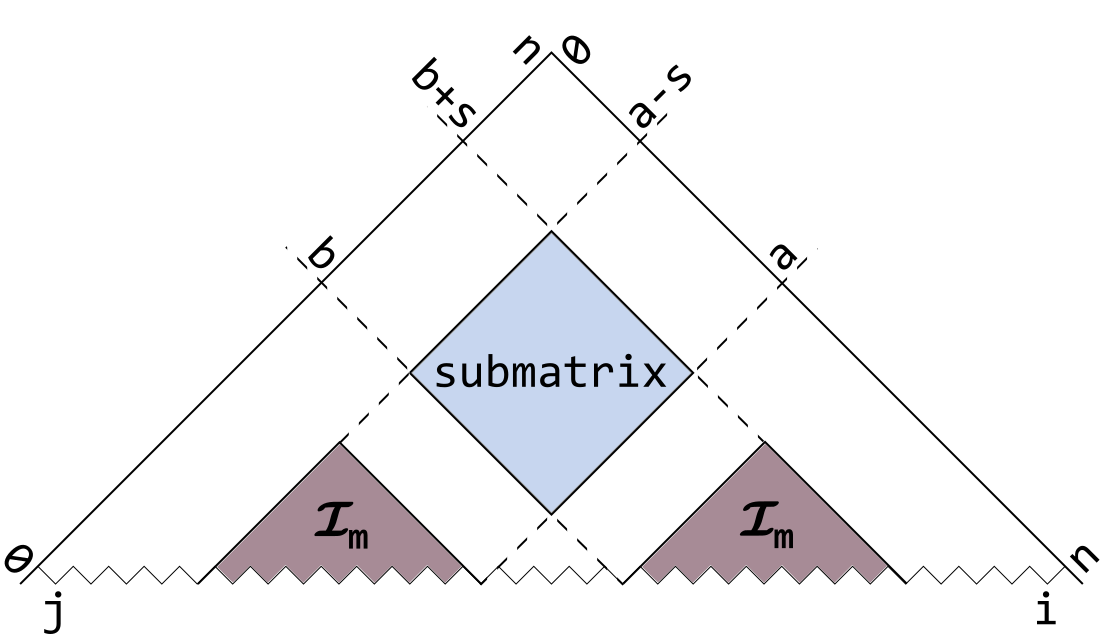
\includegraphics[width=0.9\linewidth]{submatrix.png}
  \caption{Иллюстрация к определениям~\ref{def:def_1} и \ref{def:def_2}: $(a,b)$ --- вершина подматрицы submatrix размером ($s\times s$); $\mathcal{I}_m$ --- зона, влияющая на подматрицу submatrix}
  \label{gr:submatrix}
\end{figure}

\begin{definition}
Пусть $S$ --- подматрица. Будем обозначать через $T[S]$ и $P[S]$ подматрицы матриц $T$ и $P$, соответствующие множеству индексов $S$.
\end{definition}

\pagebreak

\begin{algorithm}[caption={Вспомогательные функции обработки подматриц}, label={helpers}]
function $size(m)$
function $bottomCell(m)$

function $shift(m, i, j)$

function $leftSubmatrix(m)$
function $topSubmatrix(m)$
function $rightSubmatrix(m)$
function $bottomSubmatrix(m)$

function $rightNeighbor(m)$
function $leftNeighbor(m)$
function $rightGrounded(m)$
function $leftGrounded(m)$     
\end{algorithm}

Для описания алгоритмов нам необходимо задать ряд вспомогательных функций для оперирования подматрицами. Эти функции представлены в листинге~\ref{helpers}.

Функции $size(m)$ и $bottomCell(m)$ вычисляют размер и вершину подматрицы $m$ соответственно. Следующие четыре функции $leftSubmatrix(m)$~--- $bottomSubmatrix(m)$ возвращают одну из подматриц, делящих исходную подматрицу $m$ на четыре части, как показано на рисунке \ref{gr:inner}.

\begin{figure}[!h]
  \centering
    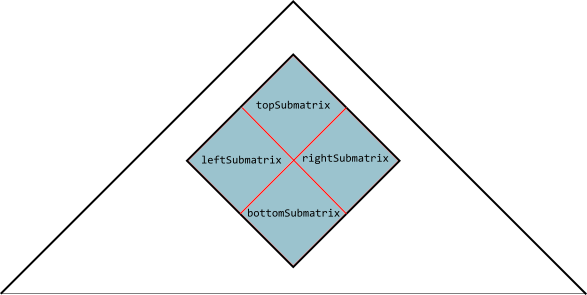
\includegraphics[width=0.9\linewidth]{inner.png}
  \caption{Иллюстрация к листингу~\ref{helpers}: разбиение матрицы на 4 компоненты}
  \label{gr:inner}
\end{figure}

Функция $shift(m, i, j)$, примененная к целым числам $i, j$ и подматрице $m$ с вершиной $(a,b)$ и размером $s$, возвращает подматрицу, сдвинутую относительно исходной на $i$ и $j$ по каждой из осей соответственно. Точнее, функция возвращает подматрицу размера $s$ с вершиной $(a+i,b+j)$. На числа $i$ и $j$ накладываются естественные ограничения основанные на том, что результирующая подматрица не может выходить за границы множества $\mathcal{I}$.

В свою очередь функции $rightNeighbor(m)$ и $leftNeighbor(m)$ возвращают подматрицы, сдвинутые относительно исходной по одной из осей, как показано на рисунке \ref{gr:outer}. Таким образом, вызов $rightNeighbor(m)$ или $leftNeighbor(m)$ эквивалентен вызову $shift(m, size(m), 0)$ или \linebreak $shift(m, 0, -size(m))$ соответственно.
Функции $rightGrounded(m)$ и \linebreak $leftGrounded(m)$ (рисунок \ref{gr:outer}) также возвращают подматрицы, сдвинутые относительно $m$, и эквивалентны вызовам функций $shift(m, b-a-1, 0)$ или $shift(m, 0, -b+a+1)$ соответственно (здесь $(a,b)$ --- вершина матрицы $m$).
Заметим, что для вершины $(i,j)$ любой их двух матриц $rightGrounded(m)$ и $leftGrounded(m)$ выполняется равенство $i + 1 = j$. Это означает, что вершина расположена в самой <<нижней>> из использующихся диагоналей всей матрицы. 

\begin{figure}[!ht]
  \centering
    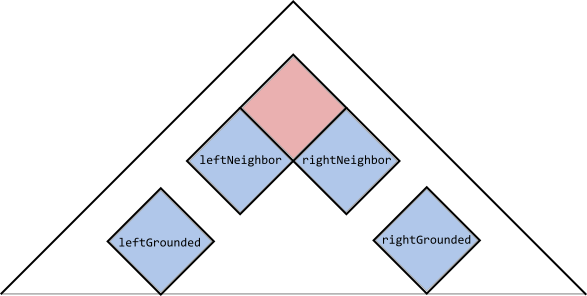
\includegraphics[width=0.9\linewidth]{outer.png}
  \caption{Иллюстрация к листингу~\ref{helpers}: соседи матрицы}
  \label{gr:outer}
\end{figure} 

Еще одна важная процедура --- \textit{performMultiplication} --- реализует основную опрацию алгоритма --- переможение подматриц. Ее тривиальная реализация представлена в листинге \ref{alg:multiplicate}. Эта процедура принимает на вход множество упорядоченных троек подматриц $(m, m_1, m_2)$ и для каждой из этих троек выполняет уножение $T[m_1] \times T[m_2]$, добавляя результат этого умножения в подматрицу $P[m]$.
% todo: умножение?

%Ниже приведён ещё один вариант кода для этой же процедуры и он сильно отличается от приведённого здесь. При чтении это смущает.

\begin{algorithm}[caption={Процедура, использующаяся для перемножения матриц}, label={alg:multiplicate}] 
procedure $performMultiplications(task)$
  foreach $(m,m_1,m_2)$ in $task$ do
    $P[m] = P[m] \cup \left(T[m_1] \times T[m_2]\right)$
\end{algorithm}

Под умножением матриц в данном случае имеется в виду операция определённая ниже. 
\begin{definition} 
Пусть $\mathcal{A},\mathcal{B}$ --- матрицы с элементами из $N$, причем $\mathcal{A}$ имеет размер $n\times k$, а $\mathcal{B}$ размер $k\times m$. Тогда результатом умножения матриц $\mathcal{A}$ и $\mathcal{B}$ является матрица $\mathcal{C}$ размера $n \times m$ с элементами из $N\times N$ и элементами, вычисленными по формуле 
$$
\mathcal{C}[i,j] = \{(A,B)\,|\,\exists k: A\in \mathcal{A}[i,k], B\in \mathcal{B}[k,j]\}.
$$
\end{definition}

\section{Алгоритм синтаксического анализа, основанный на перемножении матриц}
\label{se:okhotin}

В данном разделе описание алгоритма, взятого из статьи~\cite{okhotin13} сформулировано в определённых выше терминах и представлено в виде псевдокода, приведённого в следующем листинге~\ref{alg:okhotin}. 

Здесь, процедура $compute(i, j)$ принимает на вход такие $i, j$, что \linebreak $(i,j-1)$~--- корректная пара индексов и записывает значения во все ячейки $(i', j')$ матрицы $T$ такие, что $(i', j')$ --- корректная пара индексов, $i' \geqslant i$ и $j' < j$. 

Процедура $complete(m)$, в свою очередь, принимает на вход подматрицу $m$ и определена только для подматриц с размером, являющимся степенью двойки. $complete(m)$ вычисляет все значения матрицы $T$ на переданном ей множестве индексов $m$, при выполнении некоторых дополнительных условий. Во-первых, матрица $T$ должны быть корректно заполнена для всех пар индексов из множества $\mathcal{I}_m$. Во-вторых для всех $(i,j) \in m$ текущее значение $P[i,j]$ должно быть следующим:
$$\{(B,C)\,|\,\exists k: a < k < b;\ a_{i+1}\dots a_k \in L(B) \mbox{ и } a_{k+1}\dots a_j \in L(C)\}\,,$$
где $(a,b)$~--- вершина подматрицы $m$.

\begin{algorithm}[caption={Алгоритм синтаксического анализа, основанный на перемножении матриц}, label={alg:okhotin}] 
procedure $main()$:
  $compute(n + 1, n + 1)$
    
procedure $compute(i, j)$:
  if $j-i \geqslant 4$ then
    $compute\left(i, \frac{i+j}{2}\right)$
    $compute\left(\frac{i+j}{2}, j\right)$
  denote $m = submatrixByBottomCellAndSize\left(\left(\frac{i+j}{2}-1,\frac{i+j}{2}\right),\ \frac{j-i}{2}\right)$
  $complete(m)$
    
procedure $complete(m)$
  denote $(i, j) = bottomCell(m)$
  if $size(m) = 1$ and $i + 1 = j$ then
    $T[i,j] = \{A\,|\,A\to a_j \in R\}$
  else if $size(m) = 1$ then
    $T[i,j] = \{A\,|\,\exists (B,C) \in P[i,j]: A \to BC \in R\}$
  else if $size(m) > 1$ then
    denote $\mathcal{B} = bottomSubmatrix(m)$, $\mathcal{L} = leftSubmatrix(m)$,
           $\mathcal{R} = rightSubmatrix(m)$, $\mathcal{T} = topSubmatrix(m)$
    $complete(\mathcal{B})$
    performMultiplications($\,\{\,(\mathcal{L}, leftGrounded(\mathcal{L}), \mathcal{B})\,\}\,$)
    $complete(\mathcal{L})$
    performMultiplications($\,\{\,(\mathcal{R}, \mathcal{B}, rightGrounded(\mathcal{R}))\,\}\,$)
    $complete(\mathcal{R})$
    performMultiplications($\,\{\,(\mathcal{T}, leftGrounded(\mathcal{T}), \mathcal{R})\,\}\,$)
    performMultiplications($\,\{\,(\mathcal{T}, \mathcal{L}, rightGrounded(\mathcal{T}))\,\}\,$)
    $complete(\mathcal{T})$
\end{algorithm}

Отдельно заметим, что процедура $performMultiplications$, предназначенная, вообще говоря, для выпонения нескольких перемножений сразу, в этом алгоритме вызывается только для множеств мощности один (то есть выполняет роно одно перемножение за один вызов функции). Это накладывает ограничения на возможность параллельной реализации рассматриваемого алгоритма и предлагаемая в данной работе можификация позволяет снять эти ограничения.
% todo: ololo

\section{Модифицированный алгоритм}
\label{se:modification}

Далее предложена модификация исходного алгоритма синтаксического анализа, предназначенная для его более естественной адаптации к задаче поиска подстрок, выводимых в заданной грамматике.

Главная процедура $main$ сначала обрабатывает нижний слой матрицы $T$ (клетки $(i,j)$, для которых $i+1=j$), записывая в него корректные значения. Потом, с помощью функции $constructLayer$, разбивает матрицу $T$ на слои, как показано на рисунке \ref{gr:layers} (каждый слой состоит из набора подматриц, у каждой из которых отброшена нижняя четверть --- $bottomSubmatrix$). Полученные слои обрабатываются последовательно снизу вверх, с помощью процедуры \textit{completeVLayer}, заполняя тем самым всю матрицу $T$.

\begin{figure}[!ht]
  \centering
    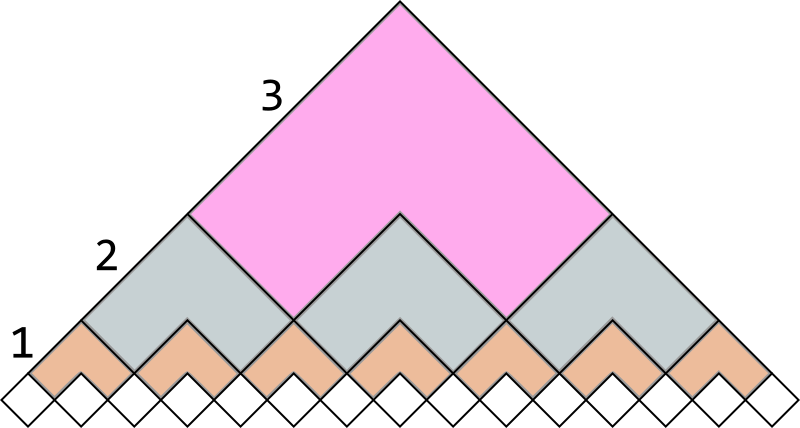
\includegraphics[width=0.9\linewidth]{layers.png}
  \caption{Первичное разбиение на слои}
  \label{gr:layers}
\end{figure}

Процедура \textit{completeVLayer}, в свою очередь, принимает на вход набор подматриц $M$. Эти подматрицы не должны пересекаться, а также для любых двух подматриц $m_1, m_2 \in M$; $(a_i,b_i),\ s_i$~--- вершина и размер $m_i$ соответственно, должно выполняться $s_1 = s_2$ и $b_1 - a_1 = b_2 - a_2$. Для каждого элемента $m$ множества $M$ процедура достраивает матрицу $T$ для трех верхних четвертей ($leftSubmatrix(m)$, $rightSubmatrix(m)$ и $topSubmatrix(m)$). Для корректной работы этой функции, во-первых, необходимо, чтобы для любой $m \in M$ ячейки $T[i,j]$ были построены  для $(i,j) \in\ bottomSubmatrix(m)$ и для $(i,j) \in\ \mathcal{I}_m$. Во-вторых, требуется выполнение ограничения на матрицу $P$, аналогичного ограничению в случае процедуры $complete$ оригинального алгоритма, а именно: для любой $m \in M$ и для всех $(i,j) \in m$ текущее значение $P[i,j]$ должно быть следующим:
$$\{(B,C)\,|\,\exists k: a < k < b;\ a_{i+1}\dots a_k \in L(B) \mbox{ и } a_{k+1}\dots a_j \in L(C)\}\,,$$
где $(a,b)$~--- вершина подматрицы $m$.

Третья процедура --- $completeLayer$ --- тоже принимает на вход набор подматриц $M$, но для каждого элемента $m$ этого набора достраивает матрицу $T$ для всей подматрицы $m$. Ограничения на входные данные такие же, как и у процедуры \textit{completeVLayer}. Для корректной работы этой функции необходимо, чтобы для любой $m \in M$ ячейки $T[i,j]$ были построены для $\mathcal{I}_m$, а так же выполнение того же требования на $P$, что и в предыдущем случае. 

\begin{algorithm}[caption={Модифицорованный алгоритм синтаксического анализа}, label={alg:modified}]
procedure $main()$:
  for $\ell$ in $\{1,\,\dots,\,n\}$ do
    $T[\ell-1, \ell] = \{A\,|\,A \to a_{\ell} \in R\}$
  foreach $1 \leqslant i < k$ do
    denote layer = $constructLayer(i)$
    $completeVLayer($layer$)$ 

procedure $constructLayer(i)$:
  denote $\mathcal{A}$ = $submatrixByBottomCellAndSize\left(\left(2^i-1,2^i\right),\ 2^i\right)$
  return $\{\mathcal{B}\,|\,\mathcal{B}\subset\mathcal{I};\,\exists k \geqslant 0:\, \mathcal{B} = shift(\mathcal{A}, k2^i, k2^i)\}$  

procedure $completeLayer(M)$:
  if $\forall\ m \in M$, $size(m) = 1$ then
    denote cells = $\{bottomCell(m)\,|\, m \in M\}$
    foreach $\{(i, j) \in $ cells $\,|\, i+1 \neq j\}$ do
      $T[i,j] = \{A\,|\,\exists (B,C) \in P[i,j]: A \to BC \in R\}$
  else
    denote bottomLayer = $\{bottomSubmatrix(m)\,|\,m \in M\}$
    $completeLayer($bottomLayer$)$
    $completeVLayer(M)$     

procedure $completeVLayer(M)$:
  denote leftSubLayer = $\{leftSubmatrix(m)\,|\,m \in M\}$
  denote rightSubLayer = $\{rightSubmatrix(m)\,|\,m \in M\}$
  denote topSubLayer = $\{topSubmatrix(m)\,|\,m \in M\}$

  denote firstMultiplicationTask = 
    $\{(m, m_1, m_2)\,|\,m \in \mbox{leftSubLayer},\,m_1 = leftGrounded(m),\,m_2 = rightNeighbor(m)\}$
    $\cup\ \{(m, m_1, m_2)\,|\,m \in \mbox{rightSubLayer},\,m_1 = leftNeighbor(m),\,m_2 = rightGrounded(m)\}$
  denote secondMultiplicationTask = 
    $\{(m, m_1, m_2)\,|\,m \in \mbox{topSubLayer},\,m_1 = leftGrounded(m),\,m_2 = rightNeighbor(m)\}$
  denote thirdMultiplicationTask = 
    $\{(m, m_1, m_2)\,|\,m \in \mbox{topSubLayer},\,m_1 = leftNeighbor(m),\,m_2 = rightGrounded(m)\}$

  $performMultiplications($firstMultiplicationTask$)$
  $completeLayer($leftSubLayer $\cup$ rightSubLayer$)$
  $performMultiplications($secondMultiplicationTask$)$
  $performMultiplications($thirdMultiplicationTask$)$
  $completeLayer($topSubLayer$)$ 
\end{algorithm}

Процедура $main$ реализуется через \textit{completeVLayer} очевидным образом. Для построения множества подматриц, составляющих слой под номером $i$, используется процедура \linebreak $constructLayer(i)$. Опишем подробнее принцип ее работы. Сначала заметим, что подматрицы уровня $i$ должны иметь размер $2^i$. Для того, чтобы построить необходимый слой сначала строится первая матрица слоя с вершиной $(2^i-1, 2^i)$ и размером $2^i$. После этого в слой добавляются все подматрицы, получающиеся из исходной сдивигом на $k*2^i, k\geqslant 0$ по каждой из осей.

Процедура $completeLayer$ по сути аналогична процедуре $complete$ из алгоритма, взятого за основу, за исключением того, что она выполняется сразу для нескольких матриц. Основная разница состоит в том, что случай $size(m) = 1$ и $i + 1 = j$ в модифицимрованном алгоритме уже разобран (первые две строки процедуры $main$). Остается отдельно разобрать случай $size(m) = 1$ и $i + 1 \neq j$.  Иначе, матрицы разбиваются на четыре части и сначала следует рекурсивный вызов от $bottomSubmatrix$ (для всех переданных матриц), а затем вызов процедуры \textit{completeVLayer}, которая обрабатывает верхние части матриц. 

Процедура \textit{completeVLayer} для каждой из переданных матриц сначала выполняет два перемножения (соответствует 21 и 23 строкам в алгоритме из статьи), затем вызывает процедуру $completeLayer$ от $rightSubmatrix$ и $leftSubmatrix$ (22 и 24 строки оригинального алгоритма), далее выполняет оставшиеся два умножения (строки 25 и 26) и, наконец, вызывает $completeLayer$ от оставшейся части $topSubmatrix$ (строка 27).

Заметим, что процедура \textit{performMultiplications} в общем случае, в отличие от исходного алгоритма,  вызывается от множеств, состоящих из нескольких элементов.
% todo:

% Наверное надо сказать пару слов о том. почему эти алгоритмы делают одно и то же?...

\section{Параллельная реализация}
\label{se:parallel}

% все о performMultiplications

% Объяснить почему перемножения группируются оптимально?...

Рассмотрим процедуру $performMultiplications$ более подробно. Во-первых заметим, что матрица $T$ на практике может представляться в виде нескольких булевых матриц: по одной матрице $T_{A}$ на каждый нетерминал $A \in N$. Тогда значения в ячейках матрицы $T$ задаются следующим образом: $T[i,j] = \{A \in N\,|\,T_{A}[i,j] = TRUE\}$. 
Аналогично, матрица $P$ представляется в виде набора булевых матриц $P_{BC}$, по одной матрице на каждую пару нетерминалов $(B, C) \in N \times N$. 
Ее значения, в свою очередь, определяются так: $P[i,j] = \{(B,C) \in N\times N\,|\,P_{BC}[i,j] = TRUE\}$.

Исходя из этого, функция $performMultiplication$ может быть реализована так, как показано в листинге~\ref{alg:multiplicate_full}.

\begin{algorithm}[caption={Процедура, использующаяся для перемножения матриц}, label={alg:multiplicate_full}] 
procedure $performMultiplications(task)$
  foreach $(m,m_1,m_2)$ in $task$ do
    foreach $(B,C)$ in $N \times N$ do
      $P_{BC}[m] = P_{BC}[m] \cup (T_{B}[m_1] \times T_{C}[m_2])$
\end{algorithm}

Итого, количество перемножений матриц, соответствующее каждому вызову процедуры $performMultiplication$, равно мощности множества $task \times N \times N$. При этом все $n = |task \times N \times N|$ умножений независимы, то есть их можно совершать в произвольном порядке. Таким образом, возможно выполнять эти умножения параллельно без затрат на синхронизацию данных. При этом в модифицированном алгоритме, в отличие от исходного, мощность множества $task$ больше единицы, что влечет за собой б\'{о}льшую степень параллелизма. 
%todo: вообще говоря, доказать независимость.
%Да, было бы неплохо, но можно в следующей итерации.

Следет заметить, что процедура $compute$ исходного алгоритма является по сути древовидной рекурсией, в которой два рекурсивных вызова (строки 6 и 7 листинга \ref{alg:okhotin}) независимы (обрабатывают непересекающиеся множества индексов). Следовательно, их тоже можно совершать параллельно.

С точки зрения практики существует несколько различных широко распространённых платформ для параллельной реализации рассмотренных алгоритмов: (многоядерный) центральный процессор (CPU), графический процессор общего назначения (GPGPU). При этом, возможны несколько уровней примерения параллелизма: параллельное умножение двух матриц и параллельное выполнение перемножения нескольких пар матриц. 

В результате, можно рассмотреть три различных способа реализации процедуры \linebreak \textit{performMultiplications}: параллельно на GPGPU, параллельно на CPU и последовательно. Важно то, что для достижения наилучшей практической производительности необходимо комбинировать три способа в рамках одного алгоритма, а именно: матрицы очень большого размера (с количеством строк $s \geqslant M_{GPU}$) умножать на GPU, матрицы поменьше (с количеством строк $s$, назодящимся в границах $M_{Parallel} \leqslant s < M_{GPU}$) умножать параллельно на CPU и оставшиеся совсем маленькие матрицы умножать последовательно. Очевидно что, для каждого из двух алгоритмов оптимальные значения $M_{GPU}$ и $M_{Parallel}$ могут быть разными.
% А что насчёт параллельного умножения большого количества маленьких матриц на GPGPU? Оказалось медленным?

% * <anya.yaveyn@yandex.ru> 22:58:17 12 Aug 2016 UTC+0300:
% да, медленнее, чем просто параллелить.. насколько я понимаю, если размер матриц маленький (константный), то количество операций линейно от количества перемножаемых матриц и количество данных тоже линейно. и константы у этих линий не очень сильно отличаются. по-этому копировать данные в gpu получается дольше, чем перемножать. 
% 
% Хотя м б с объяснением я неправа...

Для того, чтобы проверить заявленные перимущества представленного алгоритма по возможности распараллеливания нами были реализованы исходный и модифицированный алгориты. Для умножения матриц на CPU и GPGPU используются одни и те же процедуры. По результатам ряда запусков были подобраны оптимальные значения $M_{GPU} = 64$ и $M_{Parallel} = 16$ для базового алгоритма и $M_{GPU} = 32$ и $M_{Parallel} = 1$ для модифицированного. В результате базовый алгоритм работал 7.1 и 34.3 секунды на строках длины 1023 и 2047 соответственно. Время работы модифицированного алгоритма: 5.6 и 23.2 секунды. 

\section{Заключение}

Представленная модификация алгоритма облегчает задачу написания параллельной версии алгоритма, что было проверено на практике. Однако текущая реализация не является оптимальной и необходимо работать над её улучшением. Также в дальнейшем неоюбходимо  провести более полное сравнение производительности на синтетических данных и апробацию на реальных данных.

Также, у представленной модификации есть еще одно преимущество: если мы хотим адаптировать алгоритм для задачи поиска подстроки длины не большей, чем какое-то заданное $m \ll n$, тогда нам надо строить матрицы $T$ и $P$ только для индексов $i + j \leqslant n + m$. В этом случае в оригинальном алгоритме придется производить большое количество <<холостых>> рекурсивных вызовов. В модифицированном алгоритме этого отчасти можно избежать, изменив верхнюю границу в цикле for (строка 4 листинга \ref{alg:modified}).



% * <Семён Григорьев> 17:08:40 21 Jul 2016 UTC+0300:
% Подробнее про это ты пока решила не писать или просто не успела? Или там ещё пока рано что-то писать?
% ^ <Семён Григорьев> 17:11:09 21 Jul 2016 UTC+0300:
% Просто у тебя во введении есть про то, что недостаток -- проблема с разделением на потоки, а потом как-то явно про решение этой проблемы нет. Странно выглядит.
% ^ <anya.yaveyn@yandex.ru> 23:20:02 12 Aug 2016 UTC+0300:
% На самом деле я вообще не понимаю что писать в заключении ):

\begin{thebibliography}{9}

\bibitem{okhotin13}
  Alexander Okhotin,
  ``Parsing by matrix multiplication generalized to Boolean grammars'',
  \emph{Theoretical Computer Science},
  V. 516,
  p. 101--120,
  January 2014
  

\bibitem{valiant75}
  Leslie Valiant,
  ``General context-free recognition in less than cubic time'',
  \emph{Journal of Computer and System Sciences},
  10:2 (1975),
  p. 308--314.

\bibitem{hopcroft07}
  Hopcroft J. E., Motwani R., Ullman J. D.,
  ``Introduction to automata theory, languages, and computation'',
  2007.

\end{thebibliography}

\end{document}